\documentclass{article}
% General document formatting
\usepackage[margin=0.7in]{geometry}
\usepackage[parfill]{parskip}
\usepackage[utf8]{inputenc}
\usepackage{subfig}         % side-by-side figures 
% Related to math
\usepackage{amsmath,amssymb,amsfonts,amsthm}
\usepackage{graphicx}
\usepackage{natbib}
\usepackage{wrapfig}
% \bibliographystyle{unsrtnat}


% \usepackage[math]{kurier}
\usepackage{setspace}       % \onehalfspacing and \singlespacing
\newcommand\be{\begin{equation}} % shortcut to start eq envs 
\newcommand\ee{\end{equation}}   % shortcut to end eq envs
\newcommand\ol{\overline}        % shortcut to draw overline 
\newcommand\bra{\langle}
\newcommand\ket{\rangle}

\begin{document}

\title{Relating the scales of sediment burial to the characteristics of bedload transport}
\author{Kevin Pierce}
\maketitle
\section{abstract}
Bedload transport is intermittent, meaning it should really be described as a stochastic process. 
However, changes in river bed topography driven by sediment transport are usually interpreted by assuming bedload transport is deterministic. 
This work is a first stab at modeling sediment transport and bed elevations simultaneously. 
Applying a stochastic model within a control volume, we track the number of bed particles and the number of particles in motion at any instant. 
These two populations are subject to random transitions controlled by rates of entrainment and deposition. 
Since the number of particles in motion represents the bedload transport rate, and the number of particles at rest represents the bed elevation, our stochastic model describes the joint statistics of bedload transport and bed elevations. 
From the statistics of bed elevation, the time-scales of particle burial can be extracted. 
These burial time distributions have crucial implications for the interpretations of tracer experiments. 

\section{Introduction}

%( what is the problem? ) 

The transport and storage of sediment within gravel bed rivers is important for a wide range of considerations, including river restoration \citep{Gaeuman2017}, sediment budgeting \citep{Malmon2003}, and contaminant transport \citep{Malmon2005}. In relation to these problems, predictions of sediment transport and the timescales and depths of sediment burial within riverbeds are often needed, either to confine the rate of contaminant transport, or to interpret field studies based on the movement of tracer particles as they move downstream \citep{Hassan2017, Bradley2017}. Inquiries into sediment transport and burial have a significant complication. Under typical conditions in gravel bed rivers, both sediment transport rates and bed elevations evolve through time in an apparently random way. These random variations persist even under the most controlled laboratory conditions available, which suggests that bedload rates and bed elevations should really be described statistically. 

There is another factor which compounds this difficulty: bedload transport and bed elevation changes are not independent. 
Erosion of bed material increases the number of particles in motion and decreases the bed elevation, while deposition decreases the number of particles in motion and increases the bed elevation. 
Accordingly, bedload transport and bed elevations should be considered as correlated random variables.
While one set of studies has treated bed elevation changes as a stochastic process \citep{Yang1971, Nakagawa1980, Voepel2013, Martin2014}, and another set has treated bedload transport rates as a stochastic process \citep{Sun2000, Ancey2008, Heyman2013}, these two approaches have not, to my knowledge, been fused into a joint stochastic description of bedload transport and bed elevation. 

Meanwhile, our understanding of the timescales over which sediment remains buried in the riverbed leaves many open questions. Conceptually, the burial time of sediment some depth below the bed surface can be viewed as a statistical first crossing problem \citep{Voepel, Martin2014}. A buried particle will be revealed to the flow when the bed erodes away the sediment above it. As the bed elevation fluctuates in accord with successive erosion and deposition events of individual particles, 


The time over which tracers remain buried under the bed should depend on its depth of burial and the erosion rate of sediment from the bed. Because erosion is not deterministic, the burial time of sediment lies on a wide statistical distribution. 



%( what do we know about it ? ) 


Sediment within gravel bed rivers transports, under typical flow conditions, in an alternating sequence of rests and motions \citep{Einstein1937}. When grains move, they do so by rolling, sliding, and bouncing along the bed, a state of motion referred to as bedload \citep{Einstein1950, Bagnold1973, Church2006}. Owing at least to fluid turbulence and the variable configuration of grains on the bed surface \citep{Ferreira2015}, the relative exposure of grains to the flow \citep{Egiazaroff1965, McEwan2004}, and the stability of grains against forces and torques exerted by flow against their supporting contacts with other grains \citep{Coleman1967, Vowinckel2016a}, mobility varies from one stationary grain to the next \citep{Paintal1971, Celik2011, Vowinckel2016a}. Accordingly, the mobilization of individual stationary grains is not predictable \citep{Einstein1937}, but on a population level, sampling over many turbulent fluctuations and granular configurations, the mobility of grains can be characterized statistically \citep{Einstein1950, Yano1969a, Yang1971, Nakagawa1976, Dey2018}. Similarly, the trajectories of individual moving grains are not predictable, as they are subject to unknown turbulent fluctuations and random collisions with other stationary and moving grains \citep{Einstein1937, Wiberg1985, Bialik2015}, but on a population level, motion characteristics -- velocity, travel distance, travel time -- lie on statistical distributions \citep{Yano1969a, Yang1971, Nakagawa1976, Lajeunesse2010, Fathel2015, Heyman2016}, motivating probabilistic descriptions of bedload transport rates \citep{Einstein1950, Paintal1971, Nakagawa1976, Sun2000, Cheng2004, Ancey2008, Ma2014}.

Experiments indicate that, under steady laboratory conditions, bedload rates, which are a collective property of many individual motions, also fall on statistical distributions; and when mean rates rates are relatively low, the stochastic characteristics of bedload transport are emphasized, so that bedload rates express large deviations from mean values. This implies bedload distributions have relatively heavy tails \citep{Bohm2004, Ancey2008, Singh2009}. Earlier probabilistic models of the bedload flux predicted distributions which were Poissonian, with a thin tail \citep{Crickmore1962, Sayre1965, Yano1969a}, and because the observed magnitude of bedload fluctuations depends on sampling rate \citep{Ma2014}, these thin-tailed distributions fit the classic experimental data, which were obtained at relatively low sampling rates, quite well. However, with increased technological capabilities supporting bedload experiments with higher sampling rates \citep{Bohm2004, Ancey2008, Singh2009}, it became clear that instantaneous values of the bedload flux are often very large relative to mean values, and to describe this observation, some contemporary researchers have derived bedload flux distributions with heavier tails such as the negative binomial distribution \citep{Ancey2008, Heyman2013, Ma2014}. These ammended stochastic models rely on collective feedbacks in particle entrainment: when more particles are in motion, entrainment becomes more likely. These collective effects are not described in the classic literature \citep{Paintal1971, Shen1980}, and their origin, which may be associated to different processes, such as the migration of bedforms \citep{Dhont2018} or small granular avalanches from the bed surface \citep{Heyman2013} deserves further attention. Nevertheless, experiments are convincing that bedload fluctuations are wide when sampling intervals get small, and that collective feedbacks are one way to derive realistically wide fluctuations from statistical models. The model we develop here borrows this work. 

Relative exposure is a key control on particle mobility. Stationary particles are preferentially mobilized or entrained from the bed in regions of relatively high elevation, or crests \citep{Sayre1965, Sayre1967, Yang1971, Sawai1987, Wong2007}, while moving particles tend to come to rest or deposit in regions of relatively low elevation, or troughs \citep{Sayre1965, Yang1971, Charru2004, Wong2007}. These relationships between mobility and relative bed elevation stem, in large part, from the contingence of applied fluid forces on the exposed area of grains \citep{Hofland2005, Dwivedi2012}.These theoretically expected and experimentally observed trends on the differential entrainment and deposition characteristics of bed particles on crests or in troughs are a crucial component of our model, because they provide a reverting character that implies a stable distribution of bed elevations. We hypothesize these reverting attributes of entrainment and deposition describe experimentally observed bed elevation time series, which are random and almost always normally distributed, with typical deviations from mean values of one to five representative particle diameters \citep{Crickmore1962, Yang1971, Wong2007, Singh2009, Voepel2013}, and departures from normally distributed profiles when bed material is poorly consolidated or armored \citep{Singh2009}.   
 
Likewise, the entrainment and deposition of bedload particles at a location modifies the local bed elevation. \citet{Nakagawa1980} used this correlation in a statistical model to describe the development of bedforms in time from a flat bed condition, although they did not consider the modification of entrainment and deposition rates with relative bed elevation, so their model eventually breaks down, as modelled bed elevations diverge to infinite values in absence of these negative feedbacks. Other statistical models have considered bed elevations at a location as a reverting random walk \citep{Voepel2013, Martin2014}, where the bed elevation changes up or down in random increments, and these random steps are bounded from above and below by some characteristic length, which other authors mentioned in relation to the active layer concept \citep{Wong2007, Church2017}. These random walk models have a different focus than \citet{Nakagawa1980}: they are intended to describe the random changes in bed elevation caused by erosion and deposition at some location over an equilibrium bed, rather than the incipient development of bedforms on an adjusting bed. However, they are deficient because they do not relate the scales of bed elevation changes to the scales of sediment transport from which these changes emerge. That is, within these models, there is no link between the erosion and deposition rates (time scale) of individual sediment grains, the size of sediment grains (length scale) and the rate of bed elevation change (emergent time scale) and the upper and lower bounds of bed elevations at a location (emergent length scale). In this paper, we will combine earlier modelling approaches to study this link across scales, and make a first stab at understanding sediment storage by burial as an emergent property of sediment transport. 

In this development, and in accord with previous investigations, we interpret burial as the return time from above in the bed elevation time-series \citep{Voepel2013, Martin2014, Bradley2017}. For example, if the bed elevation is $y$ at the instant a deposition occurs, shifting it to some larger value, the return time from above is the time which elaspses from this instant to the next instant the bed elevation is again $y$, with the intervening interval occupied by some sequence of a number of particle entrainment and deposition events, each occurring at random instants in the interval, but necessarily, to bring the elevation back to $y$, occurring in equal proportions. Since the temporal pattern of entrainment and deposition events is random, the return time from above, or the burial time, is also random, and it its scales emerge from the statistics of sediment transport. The burial time distribution is of special interest for tracer studies and contaminant transport, as the phenomenon of anomalous super-diffusion of tracer particles can be described in terms of it \citep{Schumer2009, Martin2012, Zhang2012}. 
However, the form of the burial time distribution is contentious. Only a handful of theoretical and experimental studies have been performed, and their findings do not show clear agreement. For example, one set of experimental and theoretical investigators have measured or considered a tempered distribution for the burial time, meaning it is a power law distribution at smaller times up until some crossover point, when it becomes exponential \citep{Zhang2012,Voepel2013}.
Other investigators measured power law distributions without any crossover to exponential behavior \cite{Martin2012,Martin2014,Olinde2015,Bradley2017}. 
\citet{Martin2012, Martin2014} are based upon the same flume experiment, while \citet{Olinde2015} was a field experiment with RFID tracers which could only measure up to 10hrs and may have failed to resolve tails. 
 

- first discuss the burial time experimentally: results have been either tempered distribution or power law
- tempered distributions are a power law with an exponential tail 
- field studies are Voepel 2013 who analyzed Habersack 2001, Olinde 2015, Bradley 2016
- Voepel 2013 saw, from RFID data of Habersack, tempered distribution with exponential crossover typically around 40-50 minutes 
- Olinde 2015 used RFID tags and saw power law distributions with tail parameters during different flow events ranging from 0.24 to 0.72. Their resolution was limited to 10hrs. 
- Bradley 2017 used RFID pit tags over a 9 year tracer study to get the best experimental resolution yet. He gets 0.67 as the tail parameter. Very heavy. Smaller means heavier. 
- laboratory studies are martin2012 and martin2014
- martin 2012 gets tail parameter 0.85 power law and develops the interpretation that anomalous diffusion is due to heavy-tailed waiting times which are induced by burial. 
- martin 2014 gets tail parameters from a quasi-2d channel with bidisperse spheres for sediment of about 1 using image analysis techniques

theoretical studies: 
-yang and sayre 1971 develop exponential return time tail on cdf according to Martin 2014 
-nakagawa and tsujimoto 1980 develop exponential tail on cdf according to Martin 2014
- Zhang 2012 assumed tempered distribution for the sake of computing anomalous diffusion
-voepel 2013 gets exponential tail on cdf with a reverting random walk model which has hard reflecting boundaries at maximum and minimum elevations
-martin 2014 gets power law tail of approx 1 or slightly steeper on cdf with a reverting random walk model which has soft reflecting boundaries at maximum and   minimum elevations. they say their distributions are not truncated because of their soft reflecting quality. They highlight their tails truncate when they inadvertantly run the simulation for not enough time. 

- my conclusion? tails from my model should be power law at least in accord with the martin 2014 experiments. CDF like 1/T
- For the interpretation of field results the statement of Bradley 2017 about two return time problems ticking simultaneously is cutting 



 For example, \citet{Voepel2013} analyzed tracer data obtained in the field by \citet{Habersack2001}, and concluded that the experimental burial time distribution was tempered, meaning it is a power law distribution at shorter timescales, and it transitions at some crossover point to an exponential distribution at longer timescales, and \citet{Voepel2013} modelled the tempered distribution using a random walk model of bed elevations with hard reflecting boundaries at the maximum and minimum bed elevations.   
In contrast, \citet{Martin2012} tracked tracers within flume experiments to determine a distribution that scaled as a power law across all burial times, with no tempered crossover, which \citet{Martin2014} modelled with a random walk model of bed elevations with soft reverting boundaries. 
Similarly, \citet{Bradley2017} analyzed 9 years of data from a bedload tracer experiment to conclude the burial time distribution scaled as a power law, with no tempered crossover. 
T

There are a few theoretical and experimental suggestions that the burial time distribution is tempered, meaning it has an initial power law scaling, which transitions at some crossover point, possibly controlled by the upper and lower bounds of the bed elevation, into a thin tailed exponential distribution \citep{Zhang2012, Voepel2013, Olinde2015, Bradley2017, Fan2017}, however, the experiments of \citet{Martin2012} seem to show a power law tail instead, and \citet{Martin2014} reproduced this observation with a random-walk model of bed elevations similar to the \citet{Voepel2013} model, but with a soft reverting character at the limits of maximum and minimum bed elevation, rather than a hard barrier. 

e will investigate this burial time distribution from a different angle, and show that, in our theoretical model, it also appears tempered, and is appropriately described by the two-parameter Pareto distribution which \citet{Bradley2017} fit to field data, and we relate the crossover time between power-law and exponential regimes to the entrainment and deposition rates which statistically characterize bedload transport.  


%( how do we solve it? ) 


To do this, we pursue a fusion of the statistical model of bedform formation by \citet{Nakagawa1980} with the \citet{Einstein1950}-inspired stochastic bedload transport theory of \citet{Ancey2008} and the empirical relationships between relative exposure and local entrainment and deposition rates obtained by \citet{Sawai1987} and \citet{Wong2007}.This fusion hinges on the concept of a control volume containing some volume of bed with particles in motion above it. All resting and moving particles are idealized as identical spheres. Within this volume, we track the coordination and dynamics of two populations: first is the number of particles at rest, which changes randomly in accord with entrainment and deposition \citep{Nakagawa1980, Turowski2009}; and second is the number of particles in motion, which changes in accord with migration into the control volume from upstream, entrainment within the control volume, deposition within the control volume, and migration out of the control volume to downstream \citep{Ancey2008}. 

Using the velocity at which particles travel, we can relate the bedload rate to the number of particles in motion \citep{Einstein1950, Charru2004, Ancey2008, Furbish2012}, and using the porosity of the bed which characterizes the number of particles per unit volume of bed, we can relate the mean bed elevation within the control volume to the number of particles at rest within it. From this conceptual basis, with a two-population stochastic model, we can obtain the joint probability distribution of the number of moving particles, which is a proxy for the bedload rate \citep{Ancey2008}, and the number of stationary particles, which is a proxy for the bed elevation \citep{Nakagawa1980}. In appropriate limits, this model reduces to both of the stochastic models it's built upon. With this conceptual picture of two populations, we can study sediment burial in terms of sediment transport, and add a new perspective to the debate around the form of distributions of sediment burial time which underlie questions of tracer diffusion and contaminant transport in gravel bed rivers.   


\section{Theoretical Development}

Within a control volume, we consider the joint stochastic dynamics of two populations which may change at any instant as a result of birth, death, and migration type processes. 
These populations are the number of moving particles within the control volume, which we denote as $n$, and the number of stationary particles within the control volume, which we denote as $m$. 
The conceptual idea is depicted in figure \ref{fig:concept}. 
Of course, both of these populations are positive integers including zero. 
Following earlier writers, we assume that bedload transport characteristics are not contingent on their past history, so we can relate the rates of population change at any instant to the populations at that instant -- the Markov hypothesis \citep{Cox1965, Ancey2008}. 
This type of two-population Markov birth-death model is commonly applied to provide statistical understanding of ecological populations \citep{Cox1965, Pielou1977, Swift2002} and chemical reactions \citep{Gardiner1983, VanKampen1992, Gillespie2007}. 
In river science, a similar two-population approach has been used to understand alluvial cover and erosion within bedrock streams \citep{Turowski2009}.

\begin{wrapfigure}{r}{0.5\textwidth}
    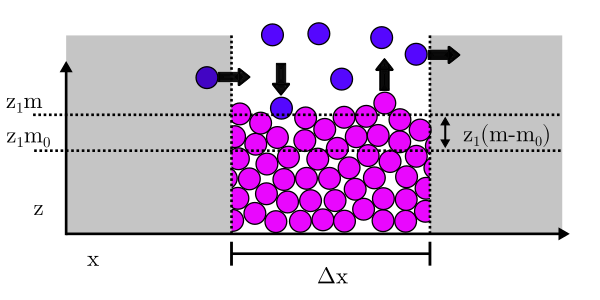
\includegraphics[width=0.5\textwidth]{./pfigures/diagram.png} %
    \caption{The conceptual picture of two populations of particles within a control volume. 
The relative bed elevation $z$ is a function of the packing fraction, particle diameter, and control volume size. 
The bed is depicted in an aggraded state where $m>m_0$. In this state, entrainment is emphasized and deposition is de-emphasized.
The four allowed transitions-- migration in, entrainment, deposition, and migration out-- are depicted with arrows. 
The system is considered independent of the adjacent system-- undoubtedly an approximation, but probably a good one for suitably large $\Delta x$. \label{fig:concept} }
\end{wrapfigure}




%\pagebreak
%\begin{figure}[h!]%
%    \centering
%    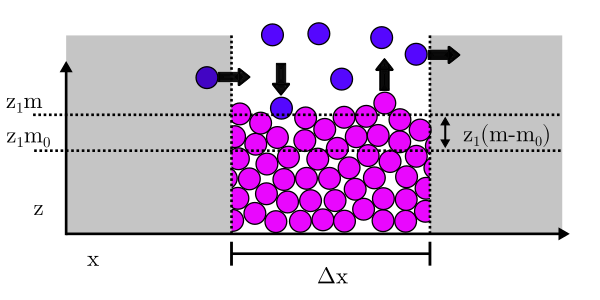
\includegraphics[width=0.5\textwidth]{./pfigures/diagram.png} %
%    \caption{The conceptual picture of two populations of particles within a control volume. 
%The relative bed elevation $z$ is a function of the packing fraction, particle diameter, and control volume size. 
%The bed is depicted in an aggraded state where $m>m_0$. In this state, entrainment is emphasized and deposition is de-emphasized.
%The four allowed transitions-- migration in, entrainment, deposition, and migration out-- are depicted with arrows. 
%The system is considered independent of the adjacent system-- undoubtedly an approximation, but probably a good one for suitably large $\Delta x$.}%
%    \label{fig:concept}%
%\end{figure}


To apply a Markov birth-death-migration model to the joint dynamics of bed elevations and bedload transport rates, we just need to outline the transitions which can modify the populations of resting and moving particles, and then specify their probabilities of occurence in a small interval of time as functions of these populations. 
Using these rates, we can consider the flow of probability through time to form a Master equation \citep{Cox1965, Pielou1977, Gardiner1983, Gillespie1992, VanKampen1992} governing the joint probability distribution $P(n,m;t)$ that there are $n$ moving particles and $m$ stationary particles within the control volume at time $t$. 
In this model, we incorporate four distinct transitions which can shift the populations at any instant: these are migration into the control volume from upstream, entrainment within the control volume, deposition within the control volume, and migration out of the control volume to downstream.
We characterize these transitions by rates, or probabilities per unit time, and by the changes they enact in the populations of moving and stationary particles within the control volume. 
The entrainment and deposition rates are expected to depend on relative bed elevation of the control volume \citep{Yang1971, Sawai1987, Wong2007}, which we relate to the number of particles at rest within the volume, and hold relative to some baseline number of particles at rest, $m_0$: 
\be z(m) = \frac{\pi a^2}{\phi \Delta x}(m-m_0) = z_1(m-m_0), \label{eq:ele}\ee
where $\Delta x$ is the downstream length of the control volume, $a$ is the radius of the idealized spherical bed particles we consider, and $\phi$ is the packing fraction of these particles, expected to be a constant value \citep{Cundall1979}. 
The factor $z_1 = \pi a^2/(\phi \Delta x)$ is an important fundamental scale of the problem. This length scale characterizes the change in elevation (in an average sense across the control volume) associated with the addition or removal of a single particle.  

Following \citet{Ancey2008}, \citet{Turowski2009}, \citet{Ancey2014a} and others, the changes in the populations these transitions enact and their probabilities of occurence in a very small time interval $dt$ can be written as
\begin{align}
\text{migration in}&   & (n,m) &\rightarrow (n+1,m)   &  &\nu dt\\
\text{entrainment}&    & (n,m) &\rightarrow (n+1,m-1) &  &[\lambda(m) + \mu(m) n]dt\\
\text{deposition}&     & (n,m) &\rightarrow (n-1,m+1) &  &\sigma(m) n dt\\
\text{migration out}&  & (n,m) &\rightarrow (n-1,m)   &  &\gamma n dt,
\end{align}
except, in a generalization of \citet{Ancey2008} to incorporate the effects of relative exposure on particle mobility, we parameterize the entrainment and deposition rates by the bed elevation \citep{Sawai1987, Wong2007}.
According to \citet{Sawai1987}, the rate of entrainment scales linearly with relative elevation, and according to \citet{Wong2007}, it scales exponentially. 
Since the linear scaling is simpler and results from the \citet{Wong2007} relationship as the limiting case of small relative bed elevations, we hold the entrainment rate linearly proportional to $z(m)$:
\begin{align}
\lambda(m) + \mu(m) n &= (\lambda_0 + \mu_0 n)\Big(1+\frac{z_1 }{(2l)^2 }z(m)\Big), & \text{entrainment rate at } (n,m). 
\end{align} 
Conceptually, the ratio $z_1/l$ controls the sensitivity of the entrainment rate to bed elevation changes. 
The additional constant factors are incorporated without loss of generality to simplify subsequent results and interpretations. 
Physically, $z_1$ is the bed elevation change induced by a single particle, and, as we will see, $l$ is related to the standard deviation of bed elevation. 
To our knowledge, there is no data about the dependence of bedload deposition rates on relative bed elevation. 
However, \citet{Wong2007} hypothesized that the scaling of deposition with bed elevation was opposite of the scaling of entrainment, and we follow this: 
\begin{align}
\sigma(m)n &= \sigma_0\Big(1-\frac{z_1}{(2l)^2  }z(m)\Big)n, & &\text{deposition rate at } (n,m).\\
\end{align}
These equations incorporate the reasonable and expected trends that entrainment happens preferentially from crests, while deposition happens preferentially from troughs. 

Using these transitions and their rates, we can write the master equation for the probability $P(n,m;t)$ that there are $n$ moving particles and $m$ stationary particles at time $t$ in the standard way \citep{Cox1965, Ancey2008}: 
\begin{multline}
 \frac{\partial P}{\partial t}(n,m;t) =  
\nu P(n-1,m;t) + 
\{\lambda(m+1) + [n-1]\mu(m+1)\}P(n-1,m+1;t)\\ + 
[n+1]\sigma(m-1)P(n+1,m-1;t) + 
[n+1]\gamma P(n+1,m;t) \\- 
\{ \nu + \lambda(m) + n\mu(m) + n\sigma(m) + n \gamma \}P(n,m;t)
. \label{eq:master}
\end{multline} 
The master equation \ref{eq:master} reduces to the master equations of \citet{Ancey2008} and \citet{Nakagawa1980} under appropriate limits. 
When $z_1/l \rightarrow 0$, meaning bed elevation changes have negligible effects on particle mobility, we obtain the \citet{Ancey2008} results for bedload transport. 
When $z_1/l \rightarrow \infty$, meaning bed elevation changes dominate particle mobility, we obtain the \citet{Nakagawa1980} results for bed elevations. 
In the intermediate region, bed elevation changes are a negative feedback on bedload transport. 

This master equation for the populations $(n,m)$ equivalently describes the probability of a given bedload rate $q_s$ and bed elevation $z(m)$, because the bedload rate, in units of number per unit time, can be written in terms of $n$ as a sum of velocities of each moving particle, $q_s = \sum_{i=1}^n u_i$, and the spatially averaged bed elevation across the control volume is related to $m$ via equation \ref{eq:ele}. 
In general, the particle velocities $u_i$ are identically distributed random variables which lie on a thin-tailed distribution \citep{Lajeunesse2010, Furbish2012, Fathel2015}, although many authors have treated them as constants \citep{Wiberg1985, Charru2004, Ancey2008}. A conflicting factor is that particles in different modes of motion (rolling, sliding, bouncing) may require separate velocity distributions under certain conditions, in order to properly characterize the transport  \citep{Frey2014}. For simplicity, we neglect these issues.

The structure of the master equation \ref{eq:master}, as an infinite system of non-linear partial differential equations, probably restricts any analytical solution for $P(n,m ;t)$. 
Furthermore, the statistical moments of $n$ and $m$ are difficult to obtain, although generating function approaches are regularly applied to similar problems \citep{Swift2002}. 
In this case, the moment equations derived from \ref{eq:master} do not close, meaning they are also an infinite hirearchy, so the problem is not much simpler than solving the original master equation. 
Accordingly, we have to take a numerical approach to proceed. 
Luckily, numerical simulation schemes for these types of population dynamics have been a topic of intense research, as there is a requirement to solve similar equations in chemical physics.
From these algorithms, weighing simplicity against efficiency, we choose the classic and straightforward stochastic simulation algorithm (SSA) of Gillespie \citep{Gillespie1977, Gillespie2007}, which simulates exact realizations (time series) of the joint population dynamics $(n(t),m(t))$, consistent with the master equation \ref{eq:master}. 
We collect many such realizations from repeated simulation, and we use this approximate ensemble to study the statistics of $n$ and $m$, i.e., of $q_s$ and $z$. 
In the next section, we present simulation results regarding the statistics of bedload transport, bed elevation changes, and their emergent property, sediment burial. 


\section{Simulation Results} 

This results are tentative, and I need to do more simulations. However, this is a start. 

\subsection{bedload transport and bed elevation}

\subsection{sediment burial} 


\section{Discussion}

\section{Conclusion} 


%\pagebreak
%\begin{figure}[h!]%
%    \centering
%    \subfloat[particle activity distribution]{{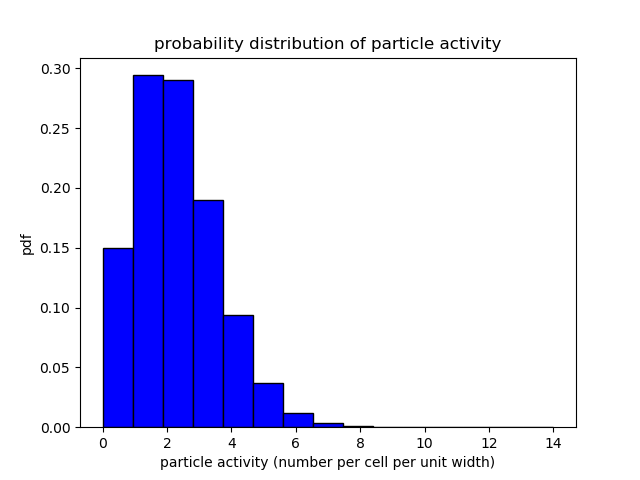
\includegraphics[width=0.45\textwidth]{activitypdf.png} }}%
%    \qquad
%    \subfloat[bed elevation distribution]{{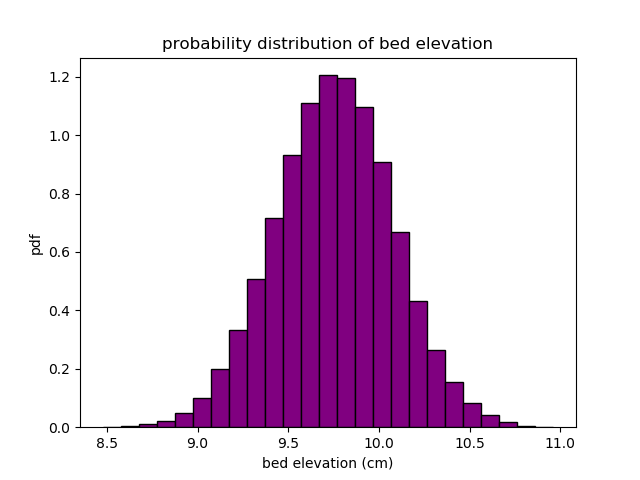
\includegraphics[width=0.45\textwidth]{elevationpdf.png} }}%
%    \caption{Particle activity and bed elevation probability distributions }%
%    \label{fig:example}%
%\end{figure}


\bibliographystyle{agu}
\bibliography{biblio}



\end{document}
